\chapter{State of the Art}
\label{State of the Art}
\thispagestyle{empty}






Introduzione al capitolo


The objective of this chapter is to illustrate more in detail the context in which our thesis is located.
In particular, the chapter is divided in two sections. First, it describes the work done by the scientific community in the field of autonomous driving, focusing expecially on reinforcement learning based algorithms.
In the second part we provide an overview of the world of autonomous driving videogames and simulators.





1. A brief history of autonomous driving

In the last decade autonomous driving has been deeply studied in several fields of research: automotive, military, racing cars, and even flight. The goal is to disrupt the need of a human driver or pilot, resulting in a reduction in costs and an increase of safety, for instance by reducing the number of accidents per year due to human error. Moreover, they could learn from their errors, and transmit to each other autonomous vehicle instantaneously, so that each of them is constantly up to date.
However, researches in the area of autonomous driving traces back to the birth of the first computers. In the '40, the scientific community were trying and gain insight about the human mind, in order to build artificial agents that could replicate -or even outperform- human in some specific tasks.
That's how computer science branched into paths such as artificial intelligence and robotics.
One of the main goal of the research of artificial intelligence has always been autonomous driving, that is the capability for an agent of perceiving the world and moving accordingly in order to reach a specific target.
Autonomous cars consists in some piece of hardware capable of moving, such as a traditional car, or a drone, equipped with some sensors give insight on the environment, one or more computer units whith a decision making algorithm, which compute an action to perform by means of some actuators, such as a throttle, a break, a steering, or a transmission.
One of the first experiments in embodying some intelligence in an artificial agent were William Grey Walter's Turtle Robots in the '50s. They were capable of moving in the sorroundings by sensing the environment in a simplified manner. They consisted in front wheel drive tricycle-like robots covered by a clear plastic shell, and were provided with a photocell and a bump detector as sensors, which resulted in the action of a motor. Despite their simple behaviors, the technique Walter used are reflected in today's reactive and biologically-inspired robots such as those based on the B.E.A.M philosophy.
Later on, in 1989, a new tentative of building an autonomous car was ALVINN, which stands for Autonomous Land Vehicle In a Neural Network, developed for military research.
At that time the technology was not sophisticated enough to provide the computation required to drive in real time, but in a sense the premise of the algorithm used nowadays was already there. In fact, neural networks are today the essential tools for building an autonomous car.
Later on with the advent of more and more sophisticated electronic components, such as sensors (Lidars and Radars, which are capable of scanning the environment at 360 degree via electromagnetic waves), and with the continuous improvement of electronic components, such as GPUs, autonomous driving started being a hot topic in industry beside scientific research.
In the last decade, some of the traditional automotive companies, such as BMW, Mercedes-Benz, General Motors, Audi, started investing in this reasearch providing their cars with a multitude of sensors and algorithms to make their cars autonomous. Ford is another manufacturer with deployments already in play, with self-driving vehicles being tested in Pittsburgh, Palo Alto, Miami, Washington D.C. and Detroit, with Austin, Texas joining them soon. Together with its partner Argo AI, Ford has plans to trial its fleet of self-driving cars in Austin with a view towards launching a wider-reaching autonomous taxi and delivery service in 2021.
Tesla, one of the companies founded by Elon Musk, is also making big steps forward in taking autonomy into mainstream use, both in terms of real world use cases and potential monetization of self-driving technologies. Tesla has supplied customers with more than 780,000 vehicles since launching, the majority of which arrive with pre-installed, self-driving capabilities available to users who purchase the requisite software. Tesla autonomous vehicles have logged huge levels of miles driven since their introduction, growing from 0.1 billion miles in May 2016 to an estimated 1.88 billion miles as of October 2019.
Waymo, the newborn firm from Google's Alfabet, has been carrying out successful trials of autonomous taxis in California, transporting over 6,200 people in the first month and many thousands since. They're proving a practical business case for autonomous vehicles.
Also in the U.S., Walmart is using autonomous cargo vans to deliver groceries in Arizona, while Pizza Hut is working with Toyota on a driverless electric delivery vehicle that even has a mobile kitchen in it to cook pizzas en route to your house.
Parallely, in the military field, DARPA (Defense Advanced Research Projects Agency) has been proposing every year since 2007 a challenge called DARPA Grand Challenge, in which scientist teams dare each other to reach some targets as fast as possible.
The reasons for this race to the autonomous driving are millions of possible accidents avoided per year, and a reduction of pollution and costs by sharing cars which are capable of transporting people without human intervention needed. %nel caso si può ampliare% 
This growth in the reaserach on autonomous cars led to a formalization of the levels of automation: Society of Automotive Engineers (SAE) introduced six levels of automation: level 0 is no automation, that is traditional cars we are accustomed to. With Level 1, driver assistance, relating to computer assistance of simple driving functions like the cruise control or automated braking systems. Cruise control consists in the capability of mantaining a certain target speed, whatever the slope of the road, weather condition, asphalt roughness. It can be accomplished via some speed sensors and a PID controller, there is no need of complex artificial intelligence. Automated braking systems involves stopping the car or reducing the speed whenever an object come across, be it a vehicle or a pedestrian. It requires proximity and distance sensors (ultrasonic or laser sensors) and may follow some manual rules based on thresholds. Lane Crossing Alert makes the car capable of notify whenever it crosses another lane, and can be achieved with camera sensors.
Level 2 refers to partial automation, where the vehicle assists drivers with steering or acceleration, allowing drivers to disengage from some tasks.  For example instance , Adaptive Cruise Control, Lane Keeping, or self-parking.
Level 3 concerns conditional automation, where the vehicle takes over some of the monitoring of the environment from the driver, using sensor technology like LiDAR. That's what the company Tesla is currently developing: their cars are able of moving in the surroundings but the human intervention is still required in dangerous situations.
Level 4 is high automation, where much greater control has been handed to the vehicle, which is in charge of steering, braking, accelerating, monitoring the vehicle and roads, and also responding to events like deciding when to change lanes, turn or use signals.
Level 5 is full automation. No company is currently able to reach this level of automation.
Currently, most of the cars are embodied with level 1 or 2. However, level 3 and 4 are still object of research, especially by tech companies such as Tesla and Waymo, whose promise is to reach these levels of automation in ten years, and level 5 in twenty, enabling their cars with the power of fully replacing human drivers.
The reasons why today full autonomous driving has not being implemented yet are the extremely huge amount of data required for perceiving the complex world of the urban scenario and for computing the consequent actions. In fact, in order to be able to perform this vast computations, several computers and GPUs are needed aboard on the car, resulting in cost, weight, and power consumption. This is the strategy adopted by Tesla so far, whose cars to day span from a price of 85000 dollars to 120000 dollars, and weigh about 2000kg. 
Another approach, adopted by companies such as Google, is to perform computation on remote servers in their datacenters. However, current mobile connections such as 4G, makes impractical the transmission of data provided each second by the vast amount of sensors.
In the future, the advent of 5G could be a game changer in this sense, which should provide a larger in bandwidth and more stable internet connection.
That's why the scientific community is starting downstepping the complexity of the task, trying to build autonomous agents in a closed and controlled environment. This lead to a simplification of the problem, avoiding the need of a real time mapping of the environment, and excluding unattended events such as pedestrian coming across.
Whether it's a matter of hardware or software, today such goal is still out of reach. Rather, some firms are focusing their attention on making a car which is autonomous in a specifing task. For example, good results have been achieved in keeping a lane on a highway, or stopping with a pedestrian coming across. 
Alternatively, good or complete levels of autonomy could be achieved in , where the perception part could be performed by simple sensors such as gps and odometry sensors.
An example could be a race track, such as Formula 1 tracks, where the environment is known apriori, and that's where our thesis move into.
In this paper we will tackle the problem of following a trajectory driven beforehand by a human driver on a race car and, if possible, to improve it.

2. Insight on autonomous driving techniques

Autonomous driving is a rather complex task: it requires a part of perception of the environment, a part of planning through an algorithm, and a part of control, to perform the actions by means of physical actuators. In our thesis we focused our attention on the planning part. In fact, by the help of a driving simulator, we could gather data with help of virtual sensors, and control the car by virtual actuators.
Perception is usually achieved through exploiting some sensors with software techniques.
Common sensors are: stereo-cameras, ultrasonic sensors, gps, speed encoders, radar and LiDars. The last one are the most accurate ones and the most expensive ones: they are capable of scanning the environment in 3D through lasers, and cost up to tens thousands dollars.
The data provided by the sensors, once cleansed and filtered, are processed in order to extract information. The main ones are image segmentation, which tries to identify objects from a RGB image through computer vision techniques such as SIFT or HOG algorithms and machine learning techniques, or the usage of stochastic models for combining multiple data coming from laser or sonar measurements.
Then, estimation of the world and of the position of the robot are used to build a map of the environment, which is used as reference to move into.
A powerful technique called SLAM enables to simultaneously localize the robot and build a map of the environment which it's moving into by combining data from internal and external sensors through algorithms such as Kalman Filters or Particle Filters.
In order to navigate in the world, the robot needs one or some algorithms that takes in input the state of itself and the world and produces as output an action to take.
Before machine learning and deep learning exploded, classical ai algorithms were used.
First, a discretization of the world was needed: it could be a graph or a grid map. Then, some search algorithms, which could be A*, Dijkstra were adopted to find the shortest path for reaching a certain goal.
Advanced controlling techniques which takes into account the dynamics of the vehicle can be exploited, one method being the linear quadratic controller, also known as Riccati controller. It minimizes a quadratic objective function in the state deviation and control energy while taking into account a linear model of the underlying system.
While a Riccati-controller is comparably fast, however, it does not directly allow the consideration of constraints such as obstacles or more advanced objective functions within
the optimization. Such requirements are met by a general nonlinear model predictive control (MPC) approach based on solving an optimal control problem in every time step.	

2.1 Reinforcement learning in autonomous driving

A combination of the advantages of both, the speed of the Riccati controller and the generality of MPC, can be achieved by finding a function that maps state values to
control variables, e. g., by training a deep neural network. Such a model could, for example, be learned supervised, as done for PILOTNET, or by reinforcement learning. The latter in particular led to excellent results in the training of such agents for controlling real-world systems such as robots or helicopters.
Recent work also shows promising applications of reinforcement learning for autonomous driving by making strategic decisions. 
Autonomous driving tasks where RL could be applied include: controller optimization, path planning and trajectory optimization, motion planning and dynamic path planning, development of high-level driving policies for complex navigation tasks, scenario-based policy learning for highways, intersections, merges and splits, reward learning with inverse reinforcement learning from expert data for intent prediction for traffic actors such as pedestrian, vehicles and finally learning of policies that ensures safety and perform risk estimation. Further, it turns out to be suitable in contexts of autonomous racing: the driverless racer could learn a policy that is able to outperform the performance of a human driver, or a policy taught by experts.
- Controlling an Autonomous Vehicle with Deep Reinforcement Learning
This paper https://arxiv.org/pdf/1909.12153.pdf shows an example of end-to-end reinforcement learning application to autonomous drive, using a proximal policy optimization algorithms by means of a neural network which maps the state to the controls. It learns two different policies: the driver and the stopper, and the reward is the squared proximity to a target position. The work aims at realizing the autonomous exploration of a parking lot based on deep reinforcement learning. It describes how a policy is trained to compute sophisticated control commands which depend on an estimate of the current vehicle state. This is done by designing an appropriate Markov decision process and a corresponding proximal policy optimization learning algorithm. For that purpose a simulated environment is used for data generation. Here, information about the vehicle's surrounding are measured by, e. g., laser scanners and are further extended by a rough knowledge about the geometry of the drivable area.
Here, the state is composed by: steering wheel angle and longitudinal acceleration; the state transition is made by single-track-models. The vehicle is assumed to have only one wheel at the front and back respectively, each centered between the real ones. Finally, two reward function are used in order to train a driver and a stopper function.


- CARMA: A Deep Reinforcement Learning Approach to Autonomous Driving
In this paper they experiment different setups of Deep Neural Networks, such as CNN and RNN as functions approximator of a reinfocement learning agent.
They formulate the state-space as follows: At each timestep, the agent receives an image I t of the environment, an estimate of the agent's speed, an estimate of the agent's distance to the center of the road, and an estimate of the angle between the agent's forward vector and the center of the road. At each timestep t, the agent can perform a discrete action: acceleration a = (Brake, DoNothing, Accelerate) and steer t = (TurnLef, DoNothing, TurnRight). Thus,there are a total of 9 possible actions the car can take at each timestep.
Then, they experimented different modeling approaches based on Q-Learning, involving CNN and RNN agents.


- Simulation-based reinforcement learning for autonomous driving:
This paper applies via reinforcement throughe Proximal Policy Optimization (PPO) with a contin-ous action space operating on multiple tensors of multiple shapes: a front camera, a high-level navigation command, car speed, and car acceleration. Thus, they adopted a custom policy that operates on multiple input tensors coming from one observation. They operated within the CARLA simulator. Their policy controls only the steering, while throttle is controlled via a PID controller with the speed set to a constant.
They modeled continuous actions with the Gaussian distribution.
The agent receives as its observation an RGB image from a single front camera from which extract semantic segmentation and car metrics such as speed and acceleration. The agent is also provided with high-level navigation command. 

	
3.

- Autonomous driving in racing:
Finding a racing line that allows to achieve a competitive lap-time is a key problem in real-world car racing as well as in the development of non-player characters for a commercial racing game.
The optimal racing line is defined as the line to follow to achieve the best lap-time possible on a given track with a given car. In general, finding the optimal racing line is
a common problem in real-world car racing as well as in the development of commercial racing games. The optimal racing line is the path that a driver should follow to complete a lap on a given track in the smallest amount of time possible. As the lap-time depends both on the distance raced and on the average racing speed, finding the optimal racing involves two different sub-problems: racing the shortest distance possible and racing as fast
as possible along the track.


Today there exist several racing-oriented driving simulators, along with developing environment. Some examples are AWS Deep Racer (Paper: DeepRacer: Educational Autonomous Racing Platform for Experimentation with Sim2Real Reinforcement Learning), TORCS, Racer (Development of a Car Racing Simulator Game Using Artificial Intelligence Techniques).

During the years, different attempts to achieve time-optimal racing, according with different technologies. 

- mettere una parte di come funziona l'intelligenza artificiale nei videogiochi


- Evolving the Optimal Racing Line in a High-End Racing Game
This paper shows how to encode a racing line by a set of connected Bézier curves, such that each gene defines a small portion of the racing line. Therefore, the evolution is responsible of the entire design of the racing line. In addition, the authors compare two different methods to evaluate the evolved racing line; the first one is based on testing the evolved racing lines in a racing simulator; the second one consists of estimating the performance of a racing line through a computational model.
	
- Ahura: A Heuristic-Based Racer for the Open Racing Car Simulator
This work proposes a controller called Ahura for TORCS. The controller uses five modules: steer controller, speed controller, opponent manager (it creates a map of opponents around  and finds the vacant slot to overtake), dynamic adjuster (friction, bumps), stuck manager (uses the idea proposed in to control the vehicle when it is out of the track or it has stuck somewhere.).
There are 23 parameters in Ahura that need to be determined:
1) eight parameters for the steer controller 
2) ten parameters for the speed controller 
3) five parameters for the opponent manager
They were determined by using the optimization algorithm CMA-ES: it has a good performance in continuous space, works with nonlinear systems, no constraint handling technique is required, and it is appropriate for nonseparable search spaces.


- Model predictive control Towards Time-Optimal Race Car Driving using Nonlinear MPC in
Real-Time
Model Predictive Control (MPC) is a multivariable control algorithm that uses:
an internal dynamic model of the process
a cost function J over the receding horizon
an optimization algorithm minimizing the cost function J using the control input u
Existing advanced control based attempts to minimum-time driving usually provide only offline open-loop solutions. . In this paper, instead, we directly use a one-level approach, solving the nonlinear MPC problem with an economic cost function in real-time. The tight real-time bounds imposed on computational times make it necessary to
reformulate the problem so as to allow for the use of efficient algorithms.
It provides real-world experimental results of the proposed nonlinear MPC scheme from a miniature race-car setup that is detailed in the paper. 


- Learning Drivers for TORCS through Imitation Using Supervised Methods	
In this work, Cardamone, Loiacono and Lanzi applied supervised learning to develop car controllers for The Open Car Race Simulator from the logs collected from other drivers. 
They considered two representations of the current state of the car: the set of rangefinder inputs usually employed in simulated car racing competitions, and a high-level, qualitative, representation involving basic lookahead information about the track in front of the car. Instead of predicting the typical low-level actions on the car actuators available in TORCS (namely, the steering wheel, the gas pedal, the brake pedal and the gear change), their approach predicts a target speed and the car position with respect to the track axis.
They considered two supervised learning methods, multi-layer neural networks and k-nearest neighbor classifiers, and applied them to compute a model mapping input sensors to actions which could imitate the behavior of an observed driver.

- Continuous Reinforcement Learning From Human Demonstrations With Integrated Experience Replay for Autonomous Driving


- Our work proposed different approaches to solve time-optimal racing problem in the framework of reinforcement learning. 



DQN:
 This can be overcome by using function approximators, more advanced algorithms such as Deep Q-Networks which use Neural Networks to estimate Q-values. 
Deep Q-Networks (DQN) \cite{atari} is an online algorithm which incorporates a variant of the Q-learning algorithm, by using deep neural networks as a non-linear Q function approximator over high-dimensional state spaces. In practice, the neural network predicts the value of all actions without the use of any explicit domain-specific information or hand-designed features. DQN applies experience replay technique to break the correlation between successive experience samples and also for better sample efficiency. For increased stability, two networks are used where the parameters of the target network for DQN are fixed for a number of iterations while updating the parameters of the online network. 
In practice, two models are provided: a model Q and a target model Q’.  Q’ is used for action selection and Q for action evaluation. That is: \[Q*(s_t,a_t)\approx r_t + \gamma Q(s_{t+1} \operatorname{argmax}_{a'} Q' (s_t,a_t))\]

While DQN is online, FQI is a batch algorithm. They adopted different kinds of decision trees as regression kernel and, in particular, KD-Trees, Tree Bagging, Extra-Trees and Totally Randomized Trees. The process consists in an iterative optimization problem, at which step the Q-function approximation in updated with a regression algorithm from a set of four-tuples \((x_t , u_t, r_t, x_{t+1})\), where $x_t$ is the state and $u_t$ is the action.  At the first iteration the fitted Q iteration algorithm is used in order to produce an approximation of the expected reward \(Q_1(x, u) = E_w [r(x, u, w)],\) where $w$ is a random disturbance. In this setting, the considered training set uses input/output pairs where the inputs are the state-action pairs and the outputs the observed rewards. In the subsequent iterations, only the output values of these input/output pairs are updated using the value iteration based on the Q-function produced at the preceding step and information about the reward and the successor state reached in each tuple. 







Machine learning (ML) is a process whereby a computer program learns from experience to improve its performance at a specified task. ML algorithms are often classified under one of three broad categories: supervised learning, unsupervised learning and reinforcement learning (RL). Supervised learning algorithms are based on inductive inference where the model is typically trained using labelled data to perform classification or regression, whereas unsupervised learning encompasses techniques such as density estimation or clustering
applied to unlabelled data. By contrast, in the RL paradigm an autonomous agent learns to improve its performance at an assigned task by interacting with its environment. RL agents are not told explicitly how to act by an expert; rather an agent’s performance is evaluated by a reward signal.
Roughly speaking, for each state experienced, the agent chooses an action and receives an occasional reward from its environment based on the usefulness of its decision. The goal for the agent is to maximize the cumulative rewards received over its lifetime. Gradually, the agent can increase its long-term reward by
exploiting knowledge learned about the expected utility of different state-action pairs. One of the main challenges in reinforcement learning is managing the trade-off between exploration and exploitation. To maximize the rewards it receives, an agent must exploit its knowledge by selecting actions which are
known to result in high rewards. On the other hand, to discover such beneficial actions, it has to take the risk of trying new actions which may lead to higher rewards than the current best-valued actions for each system state. In other words, the learning agent has to exploit what it already knows in order to obtain rewards, but it also has to explore the unknown in order to make better action selections in the future.




 \begin{figure}
    \centering
 	  \captionsetup{width=12cm}
      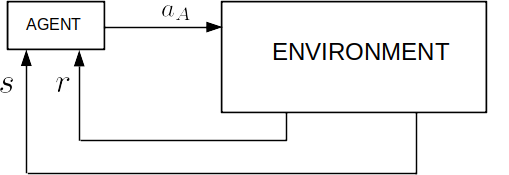
\includegraphics[width=12cm]{./img/diagram2}
     \caption{The basic RL architecture adopted in our thesis.}
   \label{fig:diagram}
  \end{figure}
As shown in Fig. \ref{fig:diagram}, an agent A produces an action $a_A$ which takes place in the environment. As a result, the agent is reward with a reward $r$ and will find itself into a new state $s$. In this simple architecture the environment is seen as a black-box, which takes as input an action and produces a reward with a new state.







\section{Controller}
